\documentclass[UTF-8,twoside,cs4size]{ctexart}
\usepackage[dvipsnames]{xcolor}
\usepackage{amsmath}
\usepackage{amssymb}
\usepackage{geometry}
\usepackage{setspace}
\usepackage{xeCJK}
\usepackage{ulem}
\usepackage{pstricks}
\usepackage{pstricks-add}
\usepackage{bm}
\usepackage{mathtools}
\usepackage{breqn}
\usepackage{mathrsfs}
\usepackage{esint}
\usepackage{textcomp}
\usepackage{upgreek}
\usepackage{pifont}
\usepackage{tikz}
\usepackage{circuitikz}
\usepackage{caption}
\usepackage{tabularx}
\usepackage{array}
\usepackage{pgfplots}
\usepackage{multirow}
\usepackage{pgfplotstable}
\usepackage{mhchem}

\newcolumntype{Y}{>{\centering\arraybackslash}X}
\geometry{a4paper,centering,top=0.75cm,bottom=2.54cm,left=2cm,right=2cm}
\pagestyle{plain}
\captionsetup{font=small}

%\CTEXsetup[name={,.}]{section}
\CTEXsetup[format={\raggedright\bfseries\noindent\zihao{3}}]{section}
\CTEXsetup[format={\raggedright\bfseries\quad\large}]{subsection}
\CTEXsetup[format={\raggedright\bfseries\qquad}]{subsubsection}
\renewcommand\thefootnote{\ding{\numexpr171+\value{footnote}}}

\setstretch{1.5}

\setCJKfamilyfont{boldsong}[AutoFakeBold = {2.17}]{SimSun}
\newcommand*{\boldsong}{\CJKfamily{boldsong}}
%\DeclareMathOperator\dif{d\!}
\newcommand*{\me}{\mathop{}\!\mathrm{e}}
\newcommand*{\mpar}{\mathop{}\!\partial}
\newcommand*{\dif}{\mathop{}\!\mathrm{d}}
\newcommand*{\tab}{\indent}
\newcommand*{\mcelsius}{\mathop{}\!{^\circ}\mathrm{C}}

\begin{document}
	\begin{flushright}
		\zihao{2}{分组号:3-07}
	\end{flushright}
	
	\noindent{\zihao{-2}\boldsong\bfseries 《\,\, 基\,\, 础\,\, 物\,\, 理\,\, 实\,\, 验\,\, 》\,\, 实\,\, 验\,\, 报\,\, 告\,\, }
	
	\noindent\textit{实验名称\uline{\quad\qquad\qquad\quad\qquad\quad 磁场的测量\,\qquad\qquad\qquad\qquad\qquad}指导教师\uline{\qquad\,\,\,刁千顺\,\,\,\qquad}}
	
	\noindent\textit{姓\qquad 名\uline{\,\,\, 桂庭辉\,\,\,}\,学号\uline{\,\,\,{\upshape2019K8009929019}\,\,\,}\,专\qquad 业\uline{\,\,\,计算机科学与技术\,\,\,}\,班级\uline{\,\,\,\upshape{03}\,\,\,}\,座号\uline{\,\,\,\upshape{6}\,\,\,}}
	
	\noindent\textit{实验日期\uline{\,\,{\upshape 2020}\,\,}年\uline{\,\,{\upshape 12}\,\,}月\uline{\,\,{\upshape23}\,\,}日\,\,实验地点\uline{\,\,\,教学楼{\upshape708}\,\,\,}调课/补课\uline{\,\,\,$ \square $是\,\,\,}成绩评定\uline{\,\,\,\quad\qquad\qquad}}
	
	\begin{table}[h]
		\centering
		\psset{linewidth=2pt}
		\begin{pspicture}(-1,-0.1)(1,0.1)
		\psline(-9,0)(9,0)
		\end{pspicture}
	\end{table}

	\begin{center}
		\Large\heiti 第一部分\quad 利用霍尔效应测量电磁铁的磁场
	\end{center}

	\section{实验目的}
	1.复习霍尔效应的基本原理;
	
	2.学习用霍尔效应测量磁场。
	
	\section{实验器材与用具}
	包含提供励磁电流和霍尔电流的电源、电流表、电压表、霍尔元件的霍尔效应实验仪,函数发生器,特斯拉计,导线,数字多用表。
	
	{\kaishu 其中,霍尔效应实验仪的主要技术指标如下:}
	
	{\kaishu 1.电磁铁励磁电流$ I_M:\,0\sim1.2\,\mathrm A $,连续可调,调节精度为1\,mA.}
	
	{\kaishu 2.霍尔元件的工作电流$ I_H:\,0\sim 11\,\mathrm{mA} $,连续可调,调节精度0.01\,mA.}
	
	{\kaishu 3.励磁电流数字表:量程为$ 0\sim 1.999\,\mathrm A $.}
	
	{\kaishu 4.霍尔电流数字表:量程为$ 0\sim 10.00\,\mathrm{mA} $.}
	
	{\kaishu 5.霍尔电压数字表:量程为$ 0\sim 199.9\,\mathrm{mV} $.}
	
	{\kaishu 6.霍尔元件材料和灵敏度:N型砷化镓,灵敏度$ K_H:\,>10\,\mathrm{V/A\cdot T} $.}
	
	{\kaishu 7.电磁铁气隙中心位置磁感应强度:$ >0.15\,\mathrm T\;(I_M=1.0\,\mathrm A) $.}
	
	{\kaishu 8.不等位电位差:$ <1\,\mathrm{mV} $(在工作电流1\,mA,磁感应强度0.1\,T时).}
	
	\section{实验原理}
	\subsection{霍尔效应}
	固体材料中的载流子在外加磁场中运动时,由于洛伦兹力的作用而运动轨迹发生偏移,在材料两侧产生电荷积累,在垂直于电流方向上形成电场,最终使得载流子所受洛伦兹力与电场力相平衡,从而在材料两侧建立起一个稳定的电势差即霍尔电压。霍尔系数为正交电场和电流强度与磁场强度乘积之比,电阻率为平行电场和电流强度之比。参与材料导电过程的不仅有带负电的电子,还有带正电的空穴。
	
	若将通有电流的导体置于磁场$ B $之中,磁场$ B $(沿$ z $轴)垂直于电流$ I_H $(沿$ x $轴)的方向,如下图所示,那么在导体中垂直于$ B $和$ I_H $的方向上出现一个横向电位差$ U_H $,这个现象称为霍尔效应。

	\begin{figure}[!h]
		\centering
		\begin{tikzpicture}
			\draw (0,0) rectangle (4,1);
			\draw (4,0)--(6,2)--(6,3)--(4,1)--cycle;
			\draw (0,1)--(2,3)--(6,3);
			\draw[dashed] (0,0)--(2,2)--(6,2);
			\draw[dashed] (2,2)--(2,3);
			\node at(2,0.5) {$ ++++++++ $};
			\node at(4,2.5) {$ -------- $};
			\draw[->] (-2,1.5)node[left]{1}--node[above,midway]{$ I_H $}(0.3,1.5);
			\draw (3,1.5)node{$ + $} circle (0.2);
			\draw[->] (2.859,1.359)--(2.577,1.077)node[left]{$ F_B $};
			\draw[->] (3.141,1.641)--(3.441,1.941)node[right]{$ F_E $};
			\draw[->] (3.2,1.5)--(4,1.5)node[right]{$ v $};
			\draw[->] (3,3.5)--(3,4.5)node[above]{$ B $};
			\draw (4.1,0)--(4.9,0);
			\draw (6.1,2)--(6.9,2);
			\draw (6.1,3)--(6.9,3);
			\draw[<->] (4.5,0)--node[right,midway]{$ w $}(6.5,2);
			\draw[<->] (6.5,2)--node[right,midway]{$ d $}(6.5,3);
			\draw[->] (5,1.5)--(7.5,1.5)node[right]{2};
			\draw (2,0.3)--(1.7,-0.5)node[below]{3};
			\draw (4.5,3)--(4.8,3.4)node[above right]{4};
			
			\draw[->] (9,-1)--(9,1)node[above]{$ z $};
			\draw[->] (9,-1)--(10.414,0.414)node[above right]{$ y $};
			\draw[->] (9,-1)--(11,-1)node[right]{$ x $};
		\end{tikzpicture}
		\caption{霍尔效应原理示意图(正电荷,空穴型)}
	\end{figure}

	当电流$ I_H $通过霍尔元件(假设为P型)时,空穴有一定的漂移速度$ v $,垂直磁场对运动电荷产生一个洛伦兹力
	\[\bm F_B=q(\bm v\times\bm B)\]
	其中$ q $为载流子电荷量。
	
	洛伦兹力将使得电荷发生横向的偏转,由于材料存在边界,所以有些偏转的载流子将会在边界积累起来,产生一个横向电场$ \bm E $,直到电场对载流子的作用力$ \bm F_E=q\bm E $与磁场作用的洛伦兹力相抵消为止,即
	\[-q(\bm v\times\bm B)=q\bm E\]
	这时起,电荷在材料中运动不再发生偏转,这个电场建立了霍尔电势差。
	
	如果是N型样品,则横向电场与前者相反,所以N型样品与P型样品的霍尔电势差有不同的符号,用于判断霍尔元件的导电类型。
	
	设P型样品的载流子浓度为$ p $,宽度为$ w $,厚度为$ d $,那么通过样品的电流$ I_H=pqvwd $,空穴的速度为
	\[v=\frac{I_H}{pqwd}\]
	从而可求得稳定后的横向电场大小为
	\[E=|\bm v\times\bm B|=\frac{I_HB}{pqwd}\]
	上式两边同时乘以$ w $即得到霍尔电势差
	\[U_H=Ew=\frac{I_HB}{pqd}=R_H\frac{I_HB}{d}=K_HI_HB\]
	其中$ R_H=\frac{1}{pq} $称为霍尔系数,$ K_H=\frac{R_H}{d}=\frac{1}{pqd} $称为霍尔元件灵敏度,单位为$ \mathrm{mV/(mA\cdot T)} $。一般而言$ K_H $越大越好,而$ K_H $与载流子浓度$ p $成反比,半导体内的载流子浓度远小于金属载流子浓度,故而常用半导体材料作为霍尔元件。又$ K_H $与厚度$ d $成反比,所以霍尔元件通常很薄,厚度一般只有0.2\,mm左右。
	
	当霍尔元件灵敏度$ K_H $已知时,只要分别测出霍尔电流$ I_H $与霍尔电势差$ U_H $,即可计算得到磁场的大小。
	
	\subsection{用霍尔效应法测量电磁铁的磁场}
	测量磁场的方法很多,例如磁通法、核磁共振法、霍尔效应法等。其中霍尔效应法用半导体材料构成霍尔片作为传感元件,将磁信号转换成电信号,测出磁场中各点的磁感应强度。其最大的优点是能测量交、直流磁场。以其为原理制成的特斯拉计能够简便、直观、快速地测量磁场。
	
	电路图如下。直流电源$ E_1 $为电磁铁提供励磁电流$ I_M $,其大小由电流表测量得到。稳压电源$ E_2 $\footnote{其可以是直流也可以是交流。}为霍尔元件提供霍尔电流$ I_H $。用毫伏表、毫安表分别测量霍尔电压、霍尔电流。励磁电流通常比霍尔电流大$ 1\sim 2 $个量级。
	
	\begin{figure}[!h]
		\centering
		\begin{circuitikz}			
			\node [ocirc] (S1) at(0,1) {};
			\draw (0,0)--(S1);
			\draw [thick] (S1)--(-0.3,1.4);
			\node [left] at(-0.3,1.25) {$ S_1 $};
			\draw (0,1.5)--(0,2.5)--(1,2.5);
			\node [ocirc] (E11) at(1,2.5) {};
			\node [ocirc] (E12) at(1.5,2.5) {};
			\node [above] at(1.25,2.5) {$ E_1 $};
			\draw (E12)--(2.5,2.5);
			\draw [thick] (2.5,-1)--(2.5,3.5);
			\draw (0,0) to[ammeter] (2.5,0);
			\draw [thick] (2.5,3.5) arc (120:60:2);
			\draw [thick] (2.5,3.5)--(3,4);
			\draw [thick] (3,4) arc (120:60:2);
			\draw [thick] (4.5,3.5)--(5,4);
			\draw [thick,-.] (4.5,3.5)--(4.5,2.3);
			\draw [thick] (4.5,2.3)--(5,2.8)--(5,4);
			\draw [thick] (4.5,2.3)--(4,2.3)--(4,2.7)--(3,2.7)--(3,-0.2);
			\draw [thick] (3,-0.2)--(3.5,0.3);
			\draw [thick] (3.5,0.3)--(3.5,2.7);
			\draw [thick] (3.5,0.3)--(4.1,0.3);
			\draw [thick] (3,-0.2)--(4,-0.2)--(4,0.2)--(4.5,0.2);
			\draw [thick] (4,0.2)--(4.5,0.7)--(5,0.7);
			\draw [thick] (5,0.7)--(4.5,0.2);
			\draw [thick] (4.5,0.2)--(4.5,-1);
			\draw [thick] (5,0.7)--(5,-0.5)--(4.5,-1);
			\draw [thick] (4.5,-1) arc (300:240:2);
			\draw (3.5,2.5)--(3,2)--(2.5,2);
			\draw (3.5,2)--(3,1.5)--(2.5,1.5);
			\draw (3.5,1.5)--(3,1)--(2.5,1);
			\draw (3.5,1)--(3,0.5)--(2.5,0.5);
			\draw (3.5,0.5)--(3,0)--(2.5,0);
			
			\draw (4,1)
			to[short,-o] (4.25,1)
			to[short] (4.5,1)
			to[short,-o] (4.75,1.25)
			to[short] (5,1.5)
			to[short,-o] (4.75,1.5)
			to[short] (4.5,1.5)
			to[short,-o] (4.25,1.25)
			to[short] (4,1);
			\draw (4.25,1)
			to[short,o-] (4.05,0.8)
			to[short] (5.1,0.8);
			\node[ocirc] (S2) at(7,0.6) {};
			\draw (4.25,1.25)
			to[short,o-] (3.8,1.25)
			to[short] (3.8,0.4)
			to[short] (5.2,0.4)
			to[voltmeter] (7,0.4)
			to[short,-o] (S2);
			\draw [thick] (S2)--(7.3,1);
			\draw (4.75,1.25)
			to[short,o-] (7,1.25)
			to[short] (7,1.1);
			\node at(7.5,0.75) {$ S_2 $};
			\draw (4.75,1.5)
			to[short,o-] (5.45,2.2)
			to[short] (5.45,4)
			to[short,-o] (6,4);
			\draw (5.1,0.8)
			to[short] (6.5,2.2)
			to[ammeter] (9,2.2)
			to[variable european resistor,a=$ R $] (9,4)
			to[short,-o] (8,4);
			\draw (6.5,4)
			to[short,o-] (7.5,4);
			\node[ocirc] (S3) at(8,4) {};
			\draw[thick] (S3)--(7.6,3.7);
			\node[above] at(7.75,4) {$ S_3 $};
			\node[above] at(6.25,4) {$ E_2 $};
		\end{circuitikz}
		\caption{霍尔效应测磁场强度电路图}
	\end{figure}
	
	半导体材料有N型(电子型)和P型(空穴型)两种,前者的载流子为电子,带负电;后者载流子为空穴,相当于带正电的粒子。若载流子为电子则4点电势高于3点,$ U_{H3,4}<0 $;若载流子为空穴则4点电势低于3点,$ U_{H3,4}>0 $。若知道载流子类型,则可以根据$ U_H $的正负判断待测磁场的方向。
	
	由于霍尔效应建立电场所需时间很短($ 10^{-12}\sim10^{-14}\,\mathrm s $),因此通过霍尔元件的电流用直流或交流都可以。若霍尔电流为交流,$ I_H=I_0\sin\omega t $,则
	\[U_H=K_HI_HB=K_HBI_0\sin\omega t\]
	得到的霍尔电压也是交变的。在使用交流电时应用$ U_H=K_HI_HB $求磁场强度时应将$ I_H,\,U_H $理解为有效值。
	
	\subsection{消除霍尔元件副效应的影响}
	实际测量过程会伴随着一些热磁副效应,使得测得的电压不只是$ U_H $,还会附加上另外一些电压,给测量带来误差。
	
	这些热磁效应应有:	
	
	{\kaishu (1)埃廷斯豪森效应,即由于在霍尔片两端有温度差,从而产生温差电动势$ U_E $,其与霍尔电流$ I_H $,磁场$ B $方向有关。如在1,2端通过电流,则在3,4端有温度差,其产生的温度梯度与通过样品的电流与磁场成正比,即3,4端方向上位置坐标为$ y $,即
	\[\frac{\mpar T}{\mpar y}=PI_HB\]
	其中$ P $称为埃廷斯豪森系数。温度梯度将引起温差电动势$ U_E $,即
	\[U_E=U(T-\Delta T,T+\Delta T)\]
	所以
	\[U_E\propto I_HB\]
	温差电动势方向与霍尔电流$ I_H $及磁场$ B $的方向有关。}
	
	{\kaishu (2)能斯特效应,即当热流通过霍尔片在其两侧会有电动势$ U_N $,只与磁场$ B $和热流有关。在P型霍尔片中,如果样品1,2端接触电阻不同,就会产生不同的焦耳热,使得两端温度不同。沿温度梯度$ \frac{\dif T}{\dif x} $有扩散倾向的空穴受到磁场的偏转,会建立一个横向电场与洛伦兹力相抗衡,则在$ y $方向电极3,4端之间产生电势差
	\[U_N=-Q\frac{\mpar T}{\mpar x}B\]
	其中$ Q $称为能斯特系数。$ U_N $的方向与磁场$ B $方向有关(热流方向一定),而与通过样品的电流$ I_H $的方向无关。}
	
	{\kaishu (3)里吉--勒迪克效应,即当热流通过霍尔片时两侧会有温度差产生,从而又产生温差电动势$ U_R $,其同样与磁场$ B $和热流有关。沿$ x $方向有温度梯度$ \frac{\mpar T}{\mpar x} $,热流沿$ x $方向通过,在$ y $方向的3,4端就会产生温度梯度,磁场方向沿$ z $方向,则有
	\[\frac{\mpar T}{\mpar y}=S\frac{\mpar T}{\mpar x}B\]
	其中$ S $称为里吉--勒迪克系数。根据埃廷斯豪森效应,在$ y $方向的温差产生温差电动势$ U_R $,与$ \frac{\mpar T}{\mpar y} $成正比,所以$ U_R $的方向随磁场$ B $的方向而改变,与霍尔电流$ I_H $无关。}

	除了这些热磁副效应外还有不等位电势差$ U_0 $,它是由与两侧(3,4端)电极不在同一等势面上引起的,当霍尔电流通过1,2端时,即便不加磁场,3,4端也会有电势差$ U_0 $产生,其方向随着$ I_H $方向改变而改变。
	
	因此为了消除副效应的影响,在操作时需分别改变$ I_H $方向和$ B $的方向,记录四组电势差数据:
	
	(1)当$ I_H $正向,$ B $正向时,$ U_1=U_H+U_0+U_E+U_N+U_R $;
	
	(2)当$ I_H $负向,$ B $正向时,$ U_2=-U_H-U_0-U_E+U_N+U_R $;
	
	(3)当$ I_H $负向,$ B $负向时,$ U_3=U_H-U_0+U_E-U_N-U_R $;
	
	(4)当$ I_H $正向,$ B $负向时,$ U_4=-U_H+U_0-U_E-U_N-U_R $.
	
	作运算$ U_1-U_2+U_3-U_4 $,并取平均值则有
	\[\frac{U_1-U_2+U_3-U_4}{4}=U_H+U_E\]
	由于$ U_E $方向始终与$ U_H $相同,故而换向法不能消除它,但一般$ U_E\ll U_H $,故而可以忽略不计,那么
	\[U_H=\frac{U_1-U_2+U_3-U_4}{4}\]
	
	此外温度差的建立时间与霍尔电势差建立时间相比较长(约几秒钟),因此如果采用交流电,可使得其来不及建立,从而实现减小误差。
	
	\section{实验内容}
	\subsection{测量霍尔电流$ I_H $与霍尔电压$ U_H $的关系}
	将霍尔片置于电磁铁中心处,设置励磁电流$ I_M=0.6\,\mathrm A $,调节霍尔电流依次为2\,mA,4\,mA,6\,mA,8\,mA,10\,mA\footnote{若电流无法加到10\,mA,加到最大即可。},测出相应的霍尔电压,每次消除副效应,作出$ U_H-I_H $图象,验证$ I_H $与$ U_H $的线性关系。
	
	\subsection{测量霍尔系数$ K_H $}
	设置霍尔电流保持$ I_H=10\,\mathrm{mA} $,由1,2端输入,将特斯拉计的探头小心地伸入电磁铁间隙中心处,调节励磁电流$ I_M $从$ 0 $至1\,A,每隔0.1\,A分别测出磁场$ B $的大小\footnote{注意磁场方向应与探头霍尔片垂直。}和样品的霍尔电压$ U_H $,每次消除副效应。用最小二乘法算出相应的$ K_H $,并求出$ K_H $的不确定度。
	
	\subsection{测量磁化曲线}
	由上小节测得的$ U_H $和求出的$ K_H $计算每个$ I_M $对应磁场$ B $的大小,从而得到磁场与励磁电流的关系$ B-I_M $曲线。
	
	\subsection{用交流霍尔电流测磁场}
	用函数发生器替代直流稳压电源$ E_2 $,设置$ f=500\,\mathrm{Hz} $,调节输出电压使得交流霍尔电流保持$ I_H=10\,\mathrm{mA} $,由1,2端输入。交流霍尔电流可用多用表的交流mA档测量。霍尔电流设定好后,将函数发生器输出直接接1,2端。用多用表测量霍尔电压$ U_H $。电磁铁的励磁电流依次为0.2\,A,0.4\,A,0.6\,A,0.8\,A,1.0\,A。算出相应的磁场,作出$ B-I_M $图象。
	
	\section{实验结果与数据处理}
	\subsection{测量霍尔电流$ I_H $与霍尔电压$ U_H $的关系}
	设置励磁电流为$ I_M=0.6\,\mathrm A $,在不同$ I_H,\;B $方向下,调节霍尔电流$ I_H $,记录数据如下\footnote{本节中所有$ U_1,\,U_2,\,U_3,\,U_4 $均取绝对值,若为负值则为与最大值方向相反,那么$ U_H $的计算方式为:
	\[U_H=\frac{U_1+U_2+U_3+U_4}{4}\]}:
	\begin{table}[!h]
		\centering
		\renewcommand\arraystretch{1.5}
		\caption{探究霍尔电流与霍尔电压关系数据记录}
		\begin{tabularx}{\textwidth}{|c|Y|Y|Y|Y|Y|}
			\hline
			\textbf{霍尔电流$ I_H\,(\mathrm{mA}) $}&$ U_1\,(\mathrm{mV}) $&$ U_2\,(\mathrm{mV}) $&$ U_3\,(\mathrm{mV}) $&$ U_4\,(\mathrm{mV}) $&$ U_H\,(\mathrm{mV}) $\\
			\hline
			\textbf{2}&2.3&2.4&4.2&4.2&3.3\\
			\hline
			\textbf{4}&4.7&4.9&8.6&8.4&6.7\\
			\hline
			\textbf{6}&7.0&7.3&13.2&12.5&10.0\\
			\hline
			\textbf{8}&9.2&9.8&17.8&16.5&13.3\\
			\hline
			\textbf{10}&11.5&12.3&22.4&20.4&16.7\\
			\hline
		\end{tabularx}
	\end{table}

	根据上表数据可作出如下拟合图象:
	\begin{figure}[!h]
		\centering
		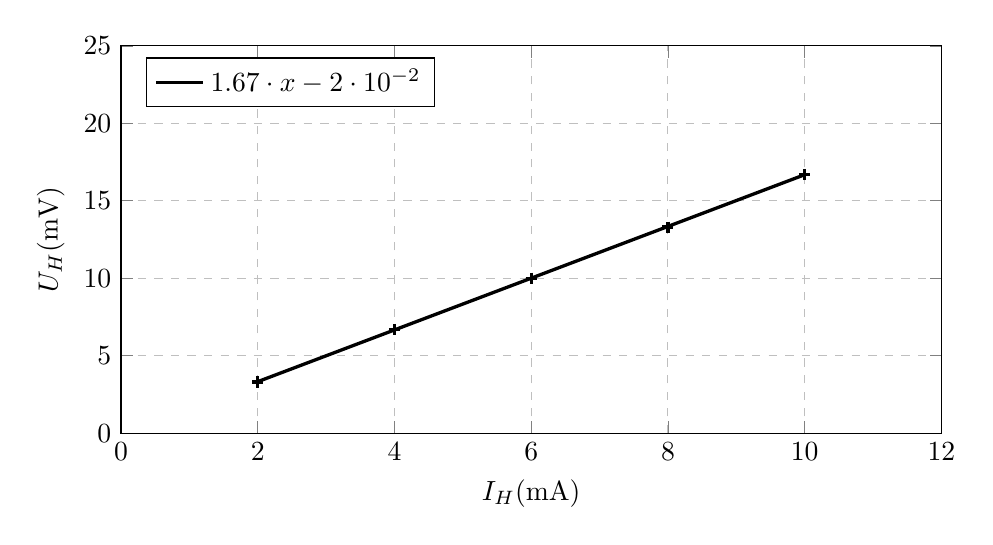
\begin{tikzpicture}
			\begin{axis}[
				legend pos=north west,
				width=12cm,height=6.5cm,
				xlabel=$ I_H(\mathrm{mA}) $,
				ylabel=$ U_H(\mathrm{mV}) $,
				xmin=0,xmax=12,
				ymin=0,ymax=25,
				xtick={0,2,4,6,8,10,12},
				ytick={0,5,10,15,20,25},
				grid style=dashed,
				ymajorgrids=true,
				xmajorgrids=true,
				]
				\addplot[no marks,black,very thick] table[y={create col/linear regression={y=Y}}]
				{
					X	Y
					2	3.3
					4	6.7
					6	10.0
					8	13.3
					10	16.7			
				};
				\addlegendentry{
					$\pgfmathprintnumber{\pgfplotstableregressiona} \cdot x
					\pgfmathprintnumber[print sign]{\pgfplotstableregressionb}$}
				
				\addplot [very thick,mark=+,only marks] coordinates {
					(2,3.3)(4,6.7)(6,10.0)(8,13.3)(10,16.7)
				};
			\end{axis}
		\end{tikzpicture}
		\caption{霍尔电流与霍尔电压关系}
	\end{figure}
	
	由上图可以看出霍尔电压与霍尔电流两者间线性关系良好。
	
	\subsection{测量霍尔系数$ K_H $}
	固定霍尔电流$ I_H=10\,\mathrm{mA} $,在不同$ I_H,\;B $方向下,调节励磁电流自$ 0 $至$ 1.0\,\mathrm{A} $。实验数据记录如下:
	
	\begin{table}[!h]
		\centering
		\renewcommand\arraystretch{1.5}
		\caption{霍尔系数测量数据记录}
		\begin{tabularx}{\textwidth}{|c|c|Y|Y|Y|Y|c|c|}
			\hline
			$ I_M\,(\mathrm A) $&$ B\,(\mathrm{mT}) $&$ U_1\,(\mathrm{mV}) $&$ U_2\,(\mathrm{mV}) $&$ U_3\,(\mathrm{mV}) $&$ U_4\,(\mathrm{mV}) $&$ U_H\,(\mathrm{mV}) $&$ K_H(\mathrm{V/(A\cdot T)}) $\\
			\hline
			\textbf{0.0}&0.4&$ -4.3 $&$ -5.0 $&5.1&4.4&0.05&12.50\\
			\hline
			\textbf{0.1}&17.2&$ -1.7 $&$ -2.1 $&7.9&7.1&2.80&16.28\\
			\hline
			\textbf{0.2}&34.3&0.8&0.8&10.8&9.7&5.5&16.03\\
			\hline
			\textbf{0.3}&51.2&3.5&3.6&13.7&12.4&8.3&16.21\\
			\hline
			\textbf{0.4}&68.6&6.1&6.5&16.6&15.1&11.08&16.14\\
			\hline
			\textbf{0.5}&85.6&8.8&9.5&19.5&17.7&13.88&16.21\\
			\hline
			\textbf{0.6}&102.7&11.4&12.4&22.4&20.3&16.63&16.19\\
			\hline
			\textbf{0.7}&119.6&14.1&15.3&25.4&23.1&19.48&16.26\\
			\hline
			\textbf{0.8}&136.9&16.8&18.2&28.3&25.7&22.25&16.25\\
			\hline
			\textbf{0.9}&153.0&19.5&21.2&31.2&28.4&25.08&16.39\\
			\hline
			\textbf{1.0}&169.6&22.2&24.1&34.1&31.0&27.85&16.42\\
			\hline
		\end{tabularx}
	\end{table}
	
	表中第一行数据计算得到的霍尔系数明显小于其他行结果,故而将其舍去,计算其他结果的平均值可得:
	\[\bar K_H=16.24\,\mathrm{V/(A\cdot T)}\]
		
	若用最小二乘法拟合处理上述数据,则可作出如下拟合图象:
	
	\begin{figure}[!h]
		\centering
		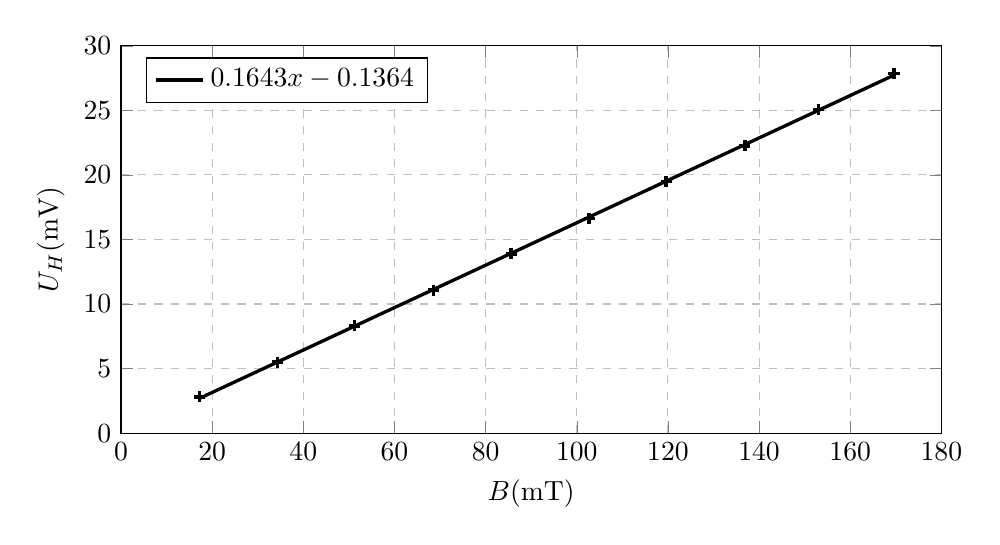
\begin{tikzpicture}
			\begin{axis}[
				legend pos=north west,
				width=12cm,height=6.5cm,
				xlabel=$ B(\mathrm{mT}) $,
				ylabel=$ U_H(\mathrm{mV}) $,
				xmin=0,xmax=180,
				ymin=0,ymax=30,
				xtick={0,20,40,60,80,100,120,140,160,180},
				ytick={0,5,10,15,20,25,30},
				grid style=dashed,
				ymajorgrids=true,
				xmajorgrids=true,
				]
				\addplot[no marks,black,very thick] table[y={create col/linear regression={y=Y}}]
				{
					X	Y
					17.2	2.80
					34.3	5.5
					51.2	8.3
					68.6	11.08
					85.6	13.88
					102.7	16.63
					119.6	19.48
					136.9	22.25
					153.0	25.08
					169.6	27.85			
				};
				\addlegendentry{
					0.1643$ x-0.1364 $}
%					$\pgfmathprintnumber{\pgfplotstableregressiona} \cdot x
%					\pgfmathprintnumber[print sign]{\pgfplotstableregressionb}$}
				
				\addplot [very thick,mark=+,only marks] coordinates {
					(17.2,2.80)(34.3,5.5)(51.2,8.3)(68.6,11.08)(85.6,13.88)(102.7,16.63)(119.6,19.48)(136.9,22.25)(153.0,25.08)(169.6,27.85)
				};
			\end{axis}
		\end{tikzpicture}
		\caption{霍尔电压与磁感应强度关系}
	\end{figure}

	拟合直线斜率$ k=K_HI_H=0.1643\,\mathrm{mV/mT} $,而$ I_H=0.01\,\mathrm A $,那么可求得
	\[K_H=\frac{k}{I_H}=16.43\,\mathrm{mV/(A\cdot mT)}=16.43\,\mathrm{V/(A\cdot T)}\]
	又$ R^2=0.9999 $,那么根据不确定度公式$ \frac{\sigma_{K_H}}{K_H}=\sqrt{\frac{1-R^2}{(n-2)R^2}} $可以计算得到
	\[\sigma_{K_H}=K_H\sqrt{\frac{1-R^2}{(n-2)R^2}}=0.0822\,\mathrm{V/(A\cdot T)}\]
	
	\subsection{测量磁化曲线}
	
	根据测得的$ U_H $,求得的$ K_H $与公式$ B=\frac{U_H}{K_HI_H} $可以计算得到不同$ I_M $对应的磁场大小如下表:
	
	\begin{table}[!h]
		\centering		
		\renewcommand\arraystretch{1.5}
		\caption{根据实验结果$ K_H $计算磁感应强度}
		\begin{tabularx}{\textwidth}{|c|Y|Y|Y|Y|Y|}
			\hline
			\textbf{励磁电流}$ I_M\,(\mathrm A) $&\textbf{0.1}&\textbf{0.2}&\textbf{0.3}&\textbf{0.4}&\textbf{0.5}\\
			\hline
			\textbf{磁感应强度}$ B\,(\mathrm{mT}) $&17.04&33.48&50.52&67.44&84.47\\
			\hline
			\textbf{励磁电流}$ I_M\,(\mathrm A) $&\textbf{0.6}&\textbf{0.7}&\textbf{0.8}&\textbf{0.9}&\textbf{1.0}\\
			\hline
			\textbf{磁感应强度}$ B\,(\mathrm{mT}) $&101.22&118.56&135.42&152.65&169.51\\
			\hline
		\end{tabularx}
	\end{table}

	根据上表数据可作出拟合图象如下页。
	
	拟合直线均方根RMSE为0.2093,即误差极小,可判定$ B $与$ I_M $成线性关系。截距$ -0.3367 $较小,忽略后可认为$ B $与$ I_M $成正比,其关系为
	\[B=kI_M,\qquad k=169.8\,\mathrm{mT/A}\]
	\newpage
	\begin{figure}[!h]
		\centering
		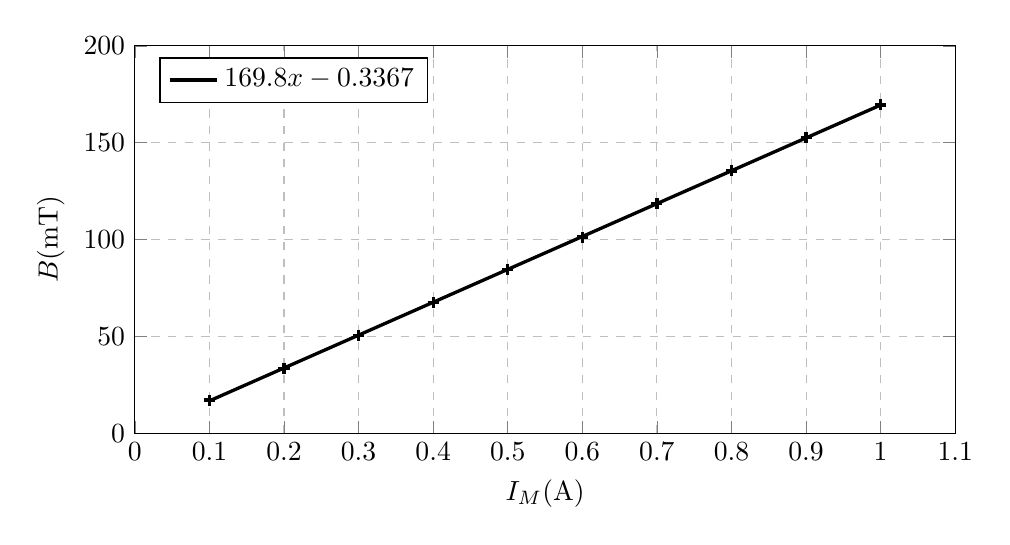
\begin{tikzpicture}
			\begin{axis}[
				legend pos=north west,
				width=12cm,height=6.5cm,
				xlabel=$ I_M(\mathrm{A}) $,
				ylabel=$ B(\mathrm{mT}) $,
				xmin=0,xmax=1.1,
				ymin=0,ymax=200,
				xtick={0,0.1,0.2,0.3,0.4,0.5,0.6,0.7,0.8,0.9,1.0,1.1},
				ytick={0,50,100,150,200},
				grid style=dashed,
				ymajorgrids=true,
				xmajorgrids=true,
				]
				\addplot[no marks,black,very thick] table[y={create col/linear regression={y=Y}}]
				{
					X	Y
					0.1	17.04
					0.2	33.48
					0.3	50.52
					0.4	67.44
					0.5	84.47
					0.6	101.22
					0.7	118.56
					0.8	135.42
					0.9	152.65
					1.0	169.51			
				};
				\addlegendentry{
					169.8$ x-0.3367 $}
%									$\pgfmathprintnumber{\pgfplotstableregressiona} \cdot x
%									\pgfmathprintnumber[print sign]{\pgfplotstableregressionb}$}
				
				\addplot [very thick,mark=+,only marks] coordinates {
					(0.1,17.04)(0.2,33.48)(0.3,50.52)(0.4,67.44)(0.5,84.47)(0.6,101.22)(0.7,118.56)(0.8,135.42)(0.9,152.65)(1.0,169.51)
				};
			\end{axis}
		\end{tikzpicture}
		\captionsetup{skip=0pt}
		\caption{$ B-I_M $图象}
	\end{figure}

	\subsection{用交流霍尔电流测磁场}
	用函数发生器替代直流稳压电源,在频率$ f=500\,\mathrm{Hz} $,交流霍尔电流有效值$ I_H=10\,\mathrm{mA} $下调节励磁电流,在$ 0.2,\,0.4,\,0.6,\,0.8,\,1.0\;\mathrm{A} $下测定相应的磁场,作出$ B-I_M $图象。
	
	复用此前由最小二乘法求得的$ K_H=16.43\,\mathrm{V/(A\cdot T)} $可通过测得的霍尔电压计算得到磁感应强度$ B $,数据记录如下:
	\begin{table}[!h]
		\centering
		\renewcommand\arraystretch{1.5}
		\caption{交流霍尔电源电压数据记录表}
		\begin{tabularx}{\textwidth}{|c|Y|Y|Y|Y|Y|}
			\hline
			\textbf{励磁电流}$ I_M(\mathrm A) $&\textbf{0.2}&\textbf{0.4}&\textbf{0.6}&\textbf{0.8}&\textbf{1.0}\\
			\hline
			\textbf{霍尔电压}$ U_H(\mathrm{mV}) $&1.0&6.1&11.6&17.1&22.7\\
			\hline
			$ B=\frac{U_H}{K_HI_H}\,(\mathrm{mT}) $&6.086&37.127&70.603&104.078&138.162\\
			\hline
		\end{tabularx}
	\end{table}
	
	那么可作出$ B-I_M $的拟合图象如下:
	
	\begin{figure}[!h]
		\centering
		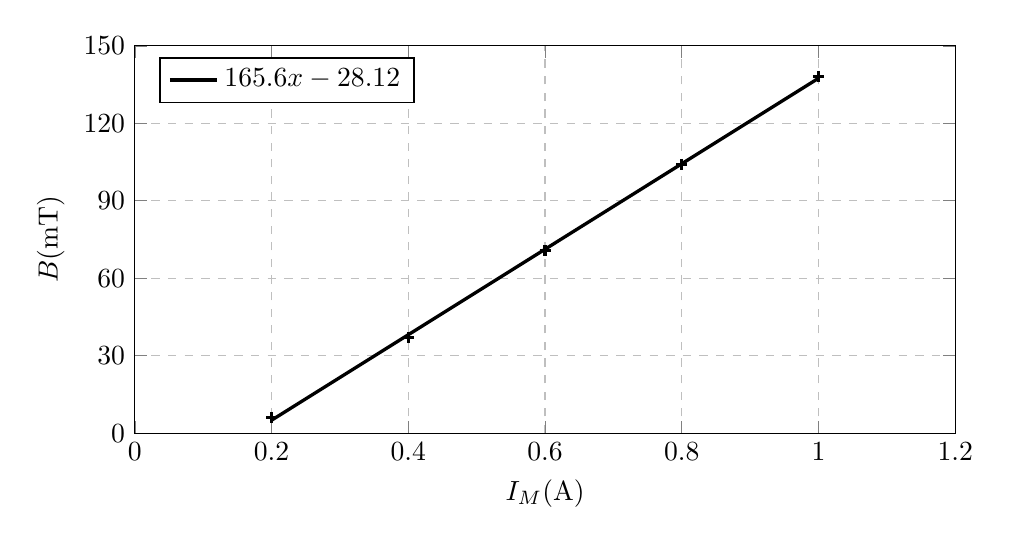
\begin{tikzpicture}
			\begin{axis}[
				legend pos=north west,
				width=12cm,height=6.5cm,
				xlabel=$ I_M(\mathrm{A}) $,
				ylabel=$ B(\mathrm{mT}) $,
				xmin=0,xmax=1.2,
				ymin=0,ymax=150,
				xtick={0,0.2,0.4,0.6,0.8,1.0,1.2},
				ytick={0,30,60,90,120,150},
				grid style=dashed,
				ymajorgrids=true,
				xmajorgrids=true,
				]
				\addplot[no marks,black,very thick] table[y={create col/linear regression={y=Y}}]
				{
					X	Y
					0.2	6.086
					0.4	37.127
					0.6	70.603
					0.8	104.078
					1.0	138.162
				};
				\addlegendentry{
					165.6$ x-28.12 $}
				%									$\pgfmathprintnumber{\pgfplotstableregressiona} \cdot x
				%									\pgfmathprintnumber[print sign]{\pgfplotstableregressionb}$}
				
				\addplot [very thick,mark=+,only marks] coordinates {
					(0.2,6.086)(0.4,37.127)(0.6,70.603)(0.8,104.078)(1.0,138.162)
				};
			\end{axis}
		\end{tikzpicture}
		\caption{交流霍尔电压下磁场强度与励磁电流拟合曲线}
	\end{figure}
	拟合直线确定系数$ R^2=0.9997 $,均方差RMSE为1.018,可认为$ B $与$ I_M $间为线性关系。
	
	\newpage
	
	~\
	
	\begin{center}
		\Large\heiti 第二部分\quad 亥姆霍兹线圈的磁场测量
	\end{center}
	\setcounter{section}{0}
	
	\section{实验目的}
	1.掌握载流圆线圈的磁场分布;
	
	2.掌握亥姆霍兹线圈的磁场分布。
	
	\section{实验仪器与用具}
	亥姆霍兹线圈磁场实验仪由亥姆霍兹线圈架部分和磁场测量仪组成。亥姆霍兹线圈架部分包括有一个传感器盒,里面装有用于测量磁场的感应线圈。
	
	{\kaishu 主要技术指标如下:}
	
	{\kaishu 1.亥姆霍兹线圈架:
		
	\tab\tab 两个励磁线圈:

	\tab\tab\tab 线圈有效半径105\,mm

	\tab\tab\tab 单个线圈匝数400匝

	\tab\tab\tab 两线圈中心间距105\,mm

	\tab\tab 移动装置:

	\tab\tab\tab 轴向可移动距离250\,mm,径向可移动距离70\,mm

	\tab\tab\tab 距离分辨率1\,mm

	\tab\tab\tab 探测线圈:匝数1000,旋转角度$ 360\,^\circ $

	2.DH4501亥姆霍兹磁场测量仪:

	\tab\tab 频率范围:$ 20\sim 200\,\mathrm{Hz} $,频率分辨率:$ 0.1\,\mathrm{Hz} $,测量误差:0.1\%

	\tab\tab 正弦波:输出电压幅度:最大$ 20\, $Vp-p,输出电流幅度:最大200\,mA

	\tab\tab 数显毫伏表电压测量范围:$ 0\sim 20\,\mathrm{mV} $,测量误差1\%

	3.电源:$ 220\,\mathrm V\pm 10\% $

	4.外形尺寸:亥姆霍兹线圈架$ 340\,\mathrm{mm}\times270\,\mathrm{mm}\times250\,\mathrm{mm} $,磁场测试仪$ 320\,\mathrm{mm}\times300\,\mathrm{mm}\times120\,\mathrm{mm} $}

	\section{实验原理}
	\subsection{载流圆线圈和亥姆霍兹线圈的磁场}
	\subsubsection{载流圆线圈的磁场}
	一半径为$ R $,通以电流$ I $的圆线圈,其轴线上磁场的公式为
	\[B=\frac{\mu_0N_0IR^2}{2(R^2+X^2)^{3/2}}\]
	其中$ N_0 $为该圆线圈的匝数,$ X $为轴上某一点到圆心$ O $的距离,$ \mu_0=4\pi\times10^{-7}\,\mathrm{H/m} $。其轴线上的磁场分布如下:
	\begin{figure}[!h]
		\centering
		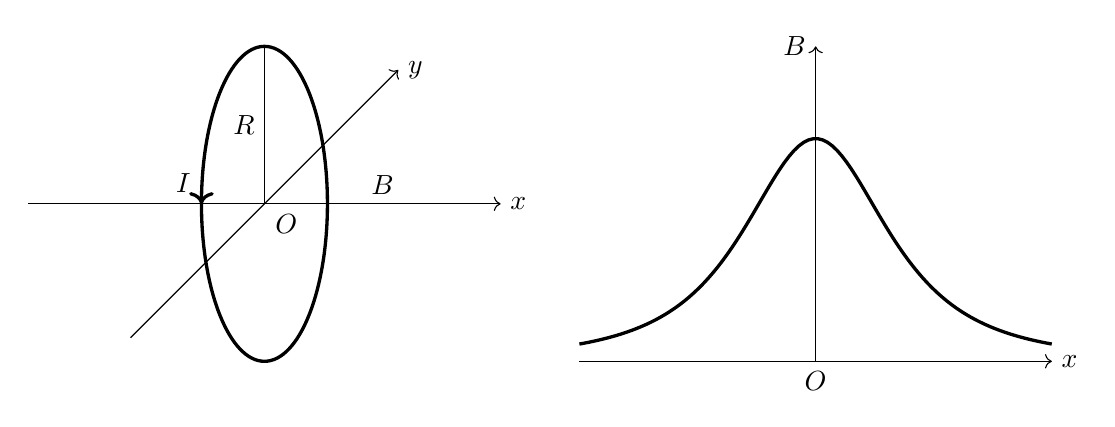
\begin{tikzpicture}
			\draw[very thick] (0,0)node[below right]{$ O $} ellipse (0.8 and 2);
			\draw[very thick,->] (-0.8,0.1)--(-0.8,0)node[above left]{$ I $};
			\draw[->] (-3,0)--(3,0)node[right]{$ x $};
			\draw (0,0)--node[left,midway]{$ R $}(0,2);
			\draw[->] (-1.7,-1.7)--(1.7,1.7)node[right]{$ y $};
			\node[above] at(1.5,0) {$ B $};
			
			\draw[->] (4,-2)--(10,-2)node[right]{$ x $};
			\draw[->] (7,-2)node[below]{$ O $}--(7,2)node[left]{$ B $};
			\draw[very thick, domain=4:10,samples=100] plot (\x,{16/(2*pow(2+pow(\x-7,2),1.5))-2});
		\end{tikzpicture}
		\caption{载流圆线圈轴向磁场分布}
	\end{figure}
	
	本实验取$ N_0=400 $匝,$ R=105\,\mathrm{mm} $。当$ f=120\,\mathrm{Hz},\;I=60\,\mathrm{mA} $\footnote{此部分实验所用$ I $均为有效值。},圆心处$ X=0 $,可计算得到单个圆线圈中的磁感应强度约为$ B=0.144\,\mathrm{mT} $.
	
	\subsubsection{亥姆霍兹线圈的磁场}
	所谓亥姆霍兹线圈彼此平行且共轴,使得线圈上通以相同方向的电流$ I $。理论计算可证明:当线圈距离$ a $等于线圈半径$ R $时,两个单线圈的磁场叠加在轴(两个线圈的圆心连线)上中点附近较大范围内的和磁场是均匀的,如下图:
	\begin{figure}[!h]
		\centering
		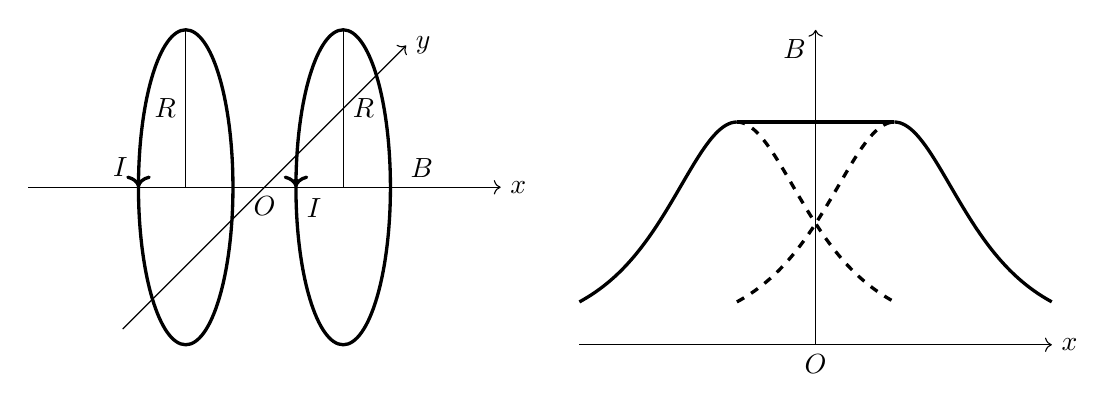
\begin{tikzpicture}
			\draw[very thick] (-1,0) ellipse (0.6 and 2);
			\draw[very thick] (1,0) ellipse (0.6 and 2);
			\draw[very thick,->] (-1.6,0.1)--(-1.6,0)node[above left]{$ I $};
			\draw[very thick,->] (0.4,0.1)--(0.4,0)node[below right]{$ I $};
			\draw[->] (-3,0)--(3,0)node[right]{$ x $};
			\draw[->] (-1.8,-1.8)--(1.8,1.8)node[right]{$ y $};
			\node[below] at(0,0) {$ O $};
			\draw (-1,0)--node[left,midway]{$ R $}(-1,2);
			\draw (1,0)--node[right,midway]{$ R $}(1,2);
			\node[above] at(2,0) {$ B $};
			
			\draw[->] (4,-2)--(10,-2)node[right]{$ x $};
			\draw[->] (7,-2)node[below]{$ O $}--(7,2)node[below left]{$ B $};
			\draw[very thick,domain=4:6,samples=100] plot (\x,{16/(2*pow(2+pow(\x-6,2),1.5))-2});
			\draw[very thick,dashed,domain=6:8,samples=100] plot (\x,{16/(2*pow(2+pow(\x-6,2),1.5))-2});
			\draw[very thick,dashed,domain=6:8,samples=100] plot (\x,{16/(2*pow(2+pow(\x-8,2),1.5))-2});
			\draw[very thick, domain=8:10,samples=100] plot (\x,{16/(2*pow(2+pow(\x-8,2),1.5))-2});
			\draw[very thick] (6,0.828)--(8,0.828);			
		\end{tikzpicture}
		\caption{亥姆霍兹线圈磁场分布}
	\end{figure}
	
	设$ z $为亥姆霍兹线圈中轴线上某一点离中心点$ O $的距离,则亥姆霍兹线圈上该点的磁感应强度为
	\[B=\frac12\mu_0NIR^2\left\{\left[R^2+\left(\frac R2+z\right)^2\right]^{-3/2}+\left[R^2+\left(\frac R2-z\right)^2\right]^{-3/2}\right\}\]
	而在亥姆霍兹线圈轴线上中心$ O $点处,$ z=0 $,则该处磁感应强度为
	\[B=\frac{\mu_0N_0I}{2R}\times\frac{16}{5^{3/2}}\]
	实验中取$ N_0=400 $匝,$ R=105\,\mathrm{mm} $。当$ f=120\,\mathrm{Hz},\;I=60\,\mathrm{mA} $时,在中心$ O $处$ z=0 $,可计算得到亥姆霍兹线圈(两个线圈的合成)磁感应强度为
	\[B=\frac{\mu_0N_0I}{2R}\times\frac{16}{5^{3/2}}=2.05\,\mathrm{mT}\]
	
	\subsection{电磁感应法测磁场}
	\subsubsection{电磁感应法测量原理}
	对于由正弦交流信号驱动的线圈产生的交变磁场,其磁场强度的瞬时值为
	\[B=B_\max\sin\omega t\]
	其中$ B_\max $为磁感应强度的峰值,其有效值为$ B $,$ \omega $为角频率。磁场中一探测线圈的磁通量为
	\[\Phi=NSB_\max\cos\theta\sin\omega t\]
	其中$ N $为探测线圈的匝数,$ S $为该线圈的截面积,$ \theta $为$ B $方向与线圈法线的夹角。线圈产生的感应电动势为
	\[\varepsilon=-\frac{\dif\Phi}{\dif t}=NS\omega B_\max\cos\theta\cos\omega t=-\varepsilon_\max\cos\omega t\]
	其中$ \varepsilon_\max=NS\omega B_\max\cos\theta $是线圈法线和磁场成$ \theta $角时感应电动势的幅值。当$ \theta=0^\circ,\;\varepsilon_\max=NS\omega B_\max $,此时感应电动势的幅值最大。如果用数字毫伏表测量此时线圈的电动势,则毫伏表的示数(即有效值)$ U_\max $为$ \frac{\varepsilon_\max}{\sqrt 2} $,则
	\[B_\max=\frac{\varepsilon_\max}{NS\omega}=\frac{\sqrt 2U_\max}{NS\omega}\]
	\subsubsection{探测线圈的设计}
	实验中由于磁场的不均匀性,而探测线圈又无法做到很小,否则会影响测量灵敏度。一般设计的线圈长度$ L $和外径$ D $有关系$ L=\frac23D $,线圈内径$ d $与外径$ D $有关系$ d\leq\frac3D $。线圈在磁场中的等效面积为
	\[S=\frac{13}{108}\pi D^2\]
	这样的线圈测得的平均磁感强度可以近似看成是中心点的磁感应强度。本实验励磁电流由专用的交变磁场测试仪提供。
	\[B=\frac{54}{13\pi^2ND^2f}U_\max\]
	将不同的频率$ f $代入上式即可计算得到$ B $,本实验$ D=0.012\,\mathrm m,\;N=1000 $匝。
	
	\section{实验内容}
	\subsection{测量圆电流线圈轴线上磁场的分布}
	调节频率调节电位器,使得频率表读数为$ 120\,\mathrm{Hz} $。调节磁场实验仪的电流调节电位器使得励磁电流有效值为$ I=60\,\mathrm{mA} $,以圆电流线圈中心为坐标原点,每隔5\,mm测一个$ U_\max $值,测量过程中注意保持励磁电流值不变,保证探测线圈法线方向与圆电流线圈轴线的夹角为$ 0^\circ $.
	\subsection{测量亥姆霍兹线圈轴线上磁场的分布}
	在励磁电流为零的情况下将磁感应强度清零。将磁场实验仪的两个线圈串联接入交流电场,调节频率电位器使得频率表读数为120\,Hz,调节磁场测量仪的电流调节电位器使得励磁电流有效值为60\,mA。以亥姆霍兹线圈中心为坐标原点,每隔5\,mm测一磁感应强度$ U_\max $的值,测量过程中注意保持励磁电流值不变。
	\subsection{测量亥姆霍兹线圈沿径向的磁场分布}
	固定探测线圈法线方向和圆电流轴线$ D $的夹角为$ 0^\circ $,转动探测线圈径向移动手轮,每隔5\,mm测量一个数据,按正负方向测到边缘,记录数据并作出磁场分布曲线图。
	\subsection{验证公式$ \varepsilon_\max=NS\omega B_\max\cos\theta $}
	当$ NS\omega B_\max $不变时,$ \varepsilon_\max $与$ \cos\theta $成正比。根据实验要求,将探测线圈沿轴线固定在某一位置上,让探测线圈法线方向与圆电流轴线的夹角从$ 0^\circ $开始,逐步转移到$ 90^\circ,\;180^\circ,\;270^\circ $,再回到$ 0^\circ $,每改变$ 10^\circ $测量一组数据。
	\subsection{励磁电流大小对磁场强度的影响}
	将探测线圈固定在亥姆霍兹线圈中心点,其法线方向与圆电流轴线$ D $夹角为$ 0^\circ $,并保持不变。调节磁场测试仪输出电流频率,在$ 20\sim 130\,\mathrm{Hz} $范围内,每次频率改变$ 10\,\mathrm{Hz} $,逐次测量感应电动势的数值并记录。
	
	\section{实验结果与数据记录}
	\subsection{测量霍尔电流$ I_H $与霍尔电压$ U_H $的关系}
	将单个圆电流线圈接入电路,轴向移动探测线圈记录不同位置下的$ U_\max $,并通过计算\footnote{根据实验原理部分,相关参数中线圈匝数$ N_0 $应使用励磁线圈匝数,即400,实验数据记录表有误。}得到数据记录表如下:
	
	\begin{table}[!h]
		\centering
		\renewcommand\arraystretch{1.5}
		\caption{圆电流线圈轴线上磁场分布数据记录}
		\small
		\begin{tabularx}{\textwidth}{|c|Y|Y|Y|Y|Y|Y|Y|Y|Y|}
			\hline
			\textbf{轴向距离}$ X(\mathrm{mm}) $&$ -35 $&$ -30 $&$ -25 $&$ -20 $&$ -15 $&$ -10 $&$ -5 $&0\\
			\hline
			$ U_\max(\mathrm{mV}) $&5.18&5.38&5.57&5.88&6.00&6.05&6.07&6.05\\
			\hline
			\textbf{测量值}$ B=\frac{2.926}{f}U_\max(\mathrm{mT}) $&0.126&0.131&0.136&0.143&0.146&0.148&0.148&0.148\\
			\hline
			\textbf{计算值}$ B=\frac{\mu_0N_0IR^2}{2(R^2+X^2)^{3/2}}(\mathrm{mT}) $&0.123&0.128&0.132&0.136&0.139&0.142&0.143&0.144\\
			\hline
			\textbf{轴向距离}$ X(\mathrm{mm}) $&5&10&15&20&25&30&35&\\
			\hline
			$ U_\max(\mathrm{mV}) $&6.05&5.98&5.88&5.75&5.60&5.41&5.20&\\
			\hline
			\textbf{测量值}$ B(\mathrm{mT}) $&0.148&0.146&0.143&0.140&0.137&0.132&0.127&\\
			\hline
			\textbf{计算值}$ B(\mathrm{mT}) $&0.143&0.142&0.139&0.136&0.132&0.128&0.123&\\
			\hline
		\end{tabularx}
	\end{table}
	
	根据上表数据可作出如下图象:
	
	\begin{figure}[!h]
		\centering
		\begin{tikzpicture}
			\begin{axis}[
				width=12cm,height=6cm,
%				title={\small (a)\;单缝衍射粗扫结果图},
				legend pos=north east,
				xlabel=$ X\;(\mathrm{mm}) $,ylabel=$ B\;(\mathrm{mT}) $,
				xmin=-40,xmax=40,
				ymin=0.120,ymax=0.160,
				xtick={-40,-30,-20,-10,-0,10,20,30,40},
				ytick={0.12,0.13,0.14,0.15,0.16},
				grid style=dashed,
				ymajorgrids=true,
				xmajorgrids=true,
				]
				\addplot [very thick,mark=*,smooth] coordinates {
					(-35,0.126)(-30,0.131)(-25,0.136)(-20,0.143)(-15,0.146)(-10,0.148)(-5,0.148)(0,0.148)(5,0.148)(10,0.146)(15,0.143)(20,0.140)(25,0.137)(30,0.132)(35,0.127)
				};
				\addlegendentry{测量值$ B $}
				
				\addplot [very thick,mark=triangle,smooth] coordinates {
					(-35,0.123)(-30,0.128)(-25,0.132)(-20,0.136)(-15,0.139)(-10,0.142)(-5,0.143)(0,0.144)(5,0.143)(10,0.142)(15,0.139)(20,0.136)(25,0.132)(30,0.128)(35,0.123)
				};
				\addlegendentry{计算值$ B $}
			\end{axis}
		\end{tikzpicture}
		\caption{圆电流线圈轴线上磁场分布}
	\end{figure}
	由上图可以看出测量值与计算值随轴向位置的变化趋势大致相同,在具体数值上测量值较计算值更大。可能的原因是探测线圈或励磁线圈的实际性能由于损耗与已知参数不同,进而得到差异较大的结果。
	
	\subsection{测量亥姆霍兹线圈轴线上磁场的分布}
	实验数据记录如下:
	\begin{table}[!h]
		\centering
		\renewcommand\arraystretch{1.5}
		\small
		\caption{亥姆霍兹线圈轴线上磁场分布数据记录}
		\begin{tabularx}{\textwidth}{|c|Y|Y|Y|Y|Y|Y|Y|Y|}
			\hline
			\textbf{轴向距离}$ X(\mathrm{mm}) $&$ -35 $&$ -30 $&$ -25 $&$ -20 $&$ -15 $&$ -10 $&$ -5 $&0\\
			\hline
			$ U_\max(\mathrm{mV}) $&8.48&8.52&8.53&8.55&8.57&8.56&8.56&8.56\\
			\hline
			\textbf{测量值}$ B=\frac{2.926}{f}U_\max(\mathrm{mT}) $&0.2069&0.2079&0.2081&0.2086&0.2091&0.2089&0.2089&0.2089\\
			\hline
			\textbf{轴向距离}$ X(\mathrm{mm}) $&5&10&15&20&25&30&35&\\
			\hline
			$ U_\max(\mathrm{mV}) $&8.55&8.56&8.56&8.57&8.55&8.52&8.49&\\
			\hline
			\textbf{测量值}$ B=\frac{2.926}{f}U_\max(\mathrm{mT}) $&0.2086&0.2089&0.2089&0.2091&0.2086&0.2079&0.2072&\\
			\hline
		\end{tabularx}
	\end{table}

	根据上表数据可作出如下图象:
	
	\begin{figure}[!h]
		\centering
		\includegraphics*[scale=0.7]{5.jpg}
		
		{\small$ y $轴为$ B(\mathrm{mT}) $,$ x $轴为$ X(\mathrm{mm}) $}
		
		\caption{亥姆霍兹线圈轴向磁场分布}
	\end{figure}
	由上图可以看出实验结果与实验原理中预期结果大致相符。
	
	\subsection{测量亥姆霍兹线圈沿径向的磁场分布}
	实验数据记录如下:
	\begin{table}[!h]
		\centering
		\renewcommand\arraystretch{1.5}
		\caption{亥姆霍兹线圈径向上磁场分布数据记录}
		\small
		\begin{tabularx}{\textwidth}{|c|Y|Y|Y|Y|Y|Y|Y|}
			\hline
			\textbf{径向距离}$ X(\mathrm{mm}) $&$ -30 $&$ -25 $&$ -20 $&$ -15 $&$ -10 $&$ -5 $&0\\
			\hline
			$ U_\max(\mathrm{mV}) $&8.52&8.53&8.54&8.55&8.56&8.56&8.56\\
			\hline
			\textbf{测量值}$ B=\frac{2.926}{f}U_\max(\mathrm{mT}) $&0.2077&0.2080&0.2082&0.2085&0.2087&0.2087&0.2087\\
			\hline
			\textbf{径向距离}$ X(\mathrm{mm}) $&5&10&15&20&25&30&\\
			\hline
			$ U_\max(\mathrm{mV}) $&8.55&8.55&8.56&8.55&8.53&8.50&\\
			\hline
			\textbf{测量值}$ B=\frac{2.926}{f}U_\max(\mathrm{mT}) $&0.2085&0.2085&0.2087&0.2085&0.2080&0.2073&\\
			\hline
		\end{tabularx}
	\end{table}
	
	根据上表数据可作出$ B-X $图象如下页.
	
	\newpage
	
	\begin{figure}[!h]
		\centering
		\includegraphics*[scale=0.8]{6.jpg}
		\caption{亥姆霍兹线圈径向磁场分布}
	\end{figure}

	由上图可以看出亥姆霍兹线圈径向磁场分布与轴向分布类似,在中点附近一定范围内磁场强度较为稳定,而离开这一定范围后磁场范围将迅速减小。
	
	\subsection{验证公式$ \varepsilon_\max=NS\omega B_\max\cos\theta $}
	实验数据记录如下:
	\begin{table}[!h]		
		\centering
		\renewcommand\arraystretch{1.5}
		\caption{探测线圈转角与感应电压数据记录}
		\small
		\begin{tabularx}{\textwidth}{|c|Y|Y|Y|Y|Y|Y|Y|Y|Y|Y|}
			\hline
			\textbf{探测线圈转角}$ \theta(^\circ) $&\textbf{0}&\textbf{10}&\textbf{20}&\textbf{30}&\textbf{40}&\textbf{50}&\textbf{60}&\textbf{70}&\textbf{80}&\textbf{90}\\
			\hline
			$ U(\mathrm{mV}) $&8.56&8.47&8.11&7.48&6.62&5.58&4.30&3.05&1.67&0.00\\
			\hline
			\textbf{计算值}$ U=U_\max\cos\theta(\mathrm{mV}) $&8.56&8.43&8.04&7.41&6.55&5.50&4.28&2.93&1.49&0.00\\
			\hline
			\textbf{探测线圈转角}$ \theta(^\circ) $&&\textbf{100}&\textbf{110}&\textbf{120}&\textbf{130}&\textbf{140}&\textbf{150}&\textbf{160}&\textbf{170}&\textbf{180}\\
			\hline
			$ U(\mathrm{mV}) $&&1.42&2.93&4.24&5.54&6.56&7.44&8.02&8.42&8.55\\
			\hline
			\textbf{计算值}$ U=U_\max\cos\theta(\mathrm{mV}) $&&1.49&2.93&4.28&5.50&6.55&7.41&8.04&8.43&8.56\\
			\hline
			\textbf{探测线圈转角}$ \theta(^\circ) $&&\textbf{190}&\textbf{200}&\textbf{210}&\textbf{220}&\textbf{230}&\textbf{240}&\textbf{250}&\textbf{260}&\textbf{270}\\
			\hline
			$ U(\mathrm{mV}) $&&8.42&8.04&7.43&6.65&5.48&4.39&3.04&1.66&0.16\\
			\hline
			\textbf{计算值}$ U=U_\max\cos\theta(\mathrm{mV}) $&&8.43&8.04&7.41&6.55&5.50&4.28&2.93&1.49&0.00\\
			\hline
			\textbf{探测线圈转角}$ \theta(^\circ) $&&\textbf{280}&\textbf{290}&\textbf{300}&\textbf{310}&\textbf{320}&\textbf{330}&\textbf{340}&\textbf{350}&\textbf{360}\\
			\hline
			$ U(\mathrm{mV}) $&&1.34&2.76&4.14&5.45&6.51&7.35&7.97&8.39&8.56\\
			\hline
			\textbf{计算值}$ U=U_\max\cos\theta(\mathrm{mV}) $&&1.49&2.93&4.28&5.50&6.55&7.41&8.04&8.43&8.56\\
			\hline
		\end{tabularx}
	\end{table}

	根据上表数据可作出图象如下页。
	
	由图象可知,实线测量值与虚线计算值重合程度较高,在误差允许范围内可看作$ U=U_\max\cos\theta $,即验证了$ \varepsilon_\max\propto\cos\theta $.
	
	~\\
	
	\begin{figure}[!h]
		\centering
		\begin{tikzpicture}
			\begin{axis}[
				width=14cm,height=10cm,
				%				title={\small (a)\;单缝衍射粗扫结果图},
				legend pos=outer north east,
				xlabel=$ \theta\;(^\circ) $,ylabel=$ U\;(\mathrm{mV}) $,
				xmin=-10,xmax=370,
				ymin=-9,ymax=9,
				xtick={0,30,60,90,120,150,180,210,240,270,300,330,360},
				ytick={-9,-6,-3,0,3,6,9},
				grid style=dashed,
				ymajorgrids=true,
				xmajorgrids=true,
				]
				\addplot [very thick,mark=+,smooth] coordinates {
					(0,8.56)(10,8.47)(20,8.11)(30,7.48)(40,6.62)(50,5.58)(60,4.30)(70,3.05)(80,1.67)(90,0)(100,-1.42)(110,-2.93)(120,-4.24)(130,-5.54)(140,-6.56)(150,-7.44)(160,-8.02)(170,-8.42)(180,-8.55)(190,-8.42)(200,-8.04)(210,-7.43)(220,-6.65)(230,-5.48)(240,-4.39)(250,-3.04)(260,-1.66)(270,-0.16)(280,1.34)(290,2.76)(300,4.14)(310,5.45)(320,6.51)(330,7.35)(340,7.97)(350,8.39)(360,8.56)
				};
				\addlegendentry{测量值$ U $}
				
				\addplot [dashed,very thick,smooth] coordinates {
					(0,8.56)(10,8.43)(20,8.04)(30,7.41)(40,6.55)(50,5.50)(60,4.28)(70,2.93)(80,1.49)(90,0.00)(100,-1.49)(110,-2.93)(120,-4.28)(130,-5.5)(140,-6.55)(150,-7.41)(160,-8.04)(170,-8.43)(180,-8.56)(190,-8.43)(200,-8.04)(210,-7.41)(220,-6.55)(230,-5.5)(240,-4.28)(250,-2.93)(260,-1.49)(270,0.00)(280,1.49)(290,2.93)(300,4.28)(310,5.5)(320,6.55)(330,7.41)(340,8.04)(350,8.43)(360,8.56)
				};
				\addlegendentry{计算值$ U $}
			\end{axis}
		\end{tikzpicture}
		\caption{验证$ U\propto\cos\theta $}
	\end{figure}
	
	\subsection{励磁电流大小对磁场强度的影响}
	实验数据记录如下:
	\begin{table}[!h]
		\centering
		\renewcommand\arraystretch{1.5}
		\caption{探究励磁电流对磁场强度影响数据记录}
		\begin{tabularx}{\textwidth}{|c|Y|Y|Y|Y|Y|Y|}
			\hline
			\textbf{励磁电流频率}$ f(\mathrm{Hz}) $&\textbf{20}&\textbf{30}&\textbf{40}&\textbf{50}&\textbf{60}&\textbf{70}\\
			\hline
			$ U_\max(\mathrm{mV}) $&1.37&2.09&2.81&3.52&4.24&4.94\\
			\hline
			\textbf{测量值}$ B=\frac{2.926}{f}U_\max(\mathrm{mT}) $&0.2004&0.2038&0.2056&0.2060&0.2068&0.2065\\
			
			\hline
			\textbf{励磁电流频率}$ f(\mathrm{Hz}) $&\textbf{80}&\textbf{90}&\textbf{100}&\textbf{110}&\textbf{120}&\textbf{130}\\
			\hline
			$ U_\max(\mathrm{mV}) $&5.66&6.38&7.11&7.82&8.56&9.27\\
			\hline
			\textbf{测量值}$ B=\frac{2.926}{f}U_\max(\mathrm{mT}) $&0.2070&0.2074&0.2080&0.2080&0.2087&0.2086\\
			\hline
		\end{tabularx}
	\end{table}
	
	根据上表数据做$ B-f $拟合直线:
	\begin{figure}[!h]
		\centering
		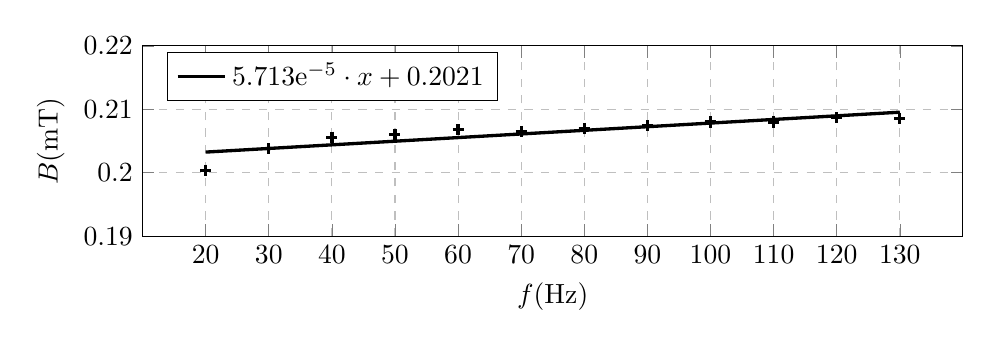
\begin{tikzpicture}
			\begin{axis}[
				legend pos=north west,
				width=12cm,height=4cm,
				xlabel=$ f(\mathrm{Hz}) $,
				ylabel=$ B(\mathrm{mT}) $,
				xmin=10,xmax=140,
				ymin=0.19,ymax=0.22,
				xtick={20,30,40,50,60,70,80,90,100,110,120,130},
				ytick={0.19,0.20,0.21,0.22},
				grid style=dashed,
				ymajorgrids=true,
				xmajorgrids=true,
				]
				\addplot[no marks,black,very thick] table[y={create col/linear regression={y=Y}}]
				{
					X	Y
					20	0.2004
					30	0.2038
					40	0.2056
					50	0.2060
					60	0.2068
					70	0.2065
					80	0.2070
					90	0.2074
					100	0.2080
					110	0.2080
					120	0.2087
					130	0.2086
				};
				\addlegendentry{
					5.713e$^{-5}\cdot x+0.2021 $}
%													$\pgfmathprintnumber{\pgfplotstableregressiona} \cdot x
%													\pgfmathprintnumber[print sign]{\pgfplotstableregressionb}$}
				
				\addplot [very thick,mark=+,only marks] coordinates {
					(20,0.2004)
					(30,0.2038)
					(40,0.2056)
					(50,0.2060)
					(60,0.2068)
					(70,0.2065)
					(80,0.2070)
					(90,0.2074)
					(100,0.2080)
					(110,0.2080)
					(120,0.2087)
					(130,0.2086)
				};
			\end{axis}
		\end{tikzpicture}
		\caption{$ B-f $拟合图象}
	\end{figure}
	
	拟合直线斜率$ 5.713\times10^{-5} $远小于$ B $测量值的量级,故而在误差允许的范围内可认为励磁电流频率$ f $不影响磁场强度。
	
	\newpage
	
	~\
	
	\begin{center}
		\Large\heiti 第三部分\quad 思考题与实验总结
	\end{center}
	\setcounter{section}{0}
	
	\section{思考题}
	\textbf{1.分析本实验主要误差来源,计算磁场$ B $的合成不确定度(分别取$ I_M=1.0\,\mathrm A,\;I_H=10\,\mathrm{mA} $)}
	
	{\kaishu 本实验误差除因实验器材本身损耗外,还来自于数字电流、电压表示数的精度,示数跳变时的读数等原因。
	
	已知:
	\begin{align*}
		K_H=16.43\,\mathrm{V/(A\cdot T)}\quad & \quad\sigma_{K_H}=0.071\,\mathrm{V/(A\cdot T)}\\
		I_H=0.01\,\mathrm{A}\quad & \quad\sigma_{I_H}=1\times10^{-5}\,\mathrm{A}\\
		U_H=0.02785\,\mathrm{V}\quad & \quad\sigma_{U_H}=1\times10^{-4}\,\mathrm A
	\end{align*}
	那么
	\begin{align*}
		\sigma_B & =\sqrt{\left(\frac{\mpar B}{\mpar K_H}\sigma_{K_H}\right)^2+\left(\frac{\mpar B}{\mpar I_H}\sigma_{I_H}\right)^2+\left(\frac{\mpar B}{\mpar U_H}\sigma_{U_H}\right)^2}\\
		& =\sqrt{(I_HU_H\sigma_{K_H})^2+(U_HK_H\sigma_{I_H})^2+(I_HK_H\sigma_{U_H})^2}\\
		& =0.0261\,\mathrm{mT}
\end{align*}}

	\textbf{2.以简图示意,用霍尔效应法判断霍尔片上的磁场方向。}
	
	{\kaishu 不妨令霍尔元件为长方体,其示意图如下:}
	\begin{figure}[!h]
		\centering
		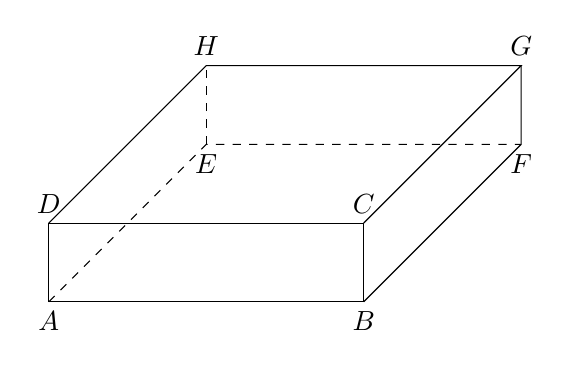
\begin{tikzpicture}
			\draw (0,0)node[below]{$ A $} rectangle (4,1)node[above]{$ C $};
			\draw (0,1)node[above]{$ D $} -- (2,3)node[above]{$ H $} -- (6,3)node[above]{$ G $} -- (4,1);
			\draw (6,3)--(6,2)node[below]{$ F $}--(4,0)node[below]{$ B $};
			\draw[dashed] (0,0)--(2,2)node[below]{$ E $}--(6,2);
			\draw[dashed] (2,2)--(2,3);
		\end{tikzpicture}
		\caption{霍尔元件简图}
	\end{figure}
	
	{\kaishu 不妨设在$ ABCD $面与$ EFGH $面之间通以电流,电流方向可由外部电路接法判断。那么可在$ ADHE $面与$ BCGF $面上通过电压表判断霍尔电压方向。若霍尔元件为P型半导体,则载流子为正电荷,运动方向与外加电流方向相同;若为N型半导体,则载流子为负电荷,运动方向与电流方向相反。最终电流稳定后载流子受力平衡,即洛伦兹力与霍尔电压产生的电场力相平衡,其方向与电场力方向相反,而电场力方向可由$ ADHE $面与$ BCGF $方向上电势差正负、载流子电性推知。已知洛伦兹力方向与载流子运动方向,则可通过矢量合成的方式判断磁场方向。}
	
	~\
	
	\textbf{3.如何测量交变磁场,写出主要步骤。}
	
	{\kaishu 将霍尔元件置于交变磁场中,将霍尔电压接在示波器上,对波形进行观察与测量即可。还可以利用交变磁场激励一个探测线圈,并将线圈接在示波器上,转动线圈至电动势峰值最大处,已知线圈匝数$ N $、面积$ S $,则可利用感生电动势公式$ E=NS\frac{\dif B}{\dif t} $对波形曲线作积分以得到交变磁场中磁感应强度与时间的关系式。}
	
	~\
	
	\textbf{4.单线圈轴线上磁场的分布规律如何?亥姆霍兹线圈是怎样组成的?其基本条件有哪些?它的磁场分布特点怎样?}
	
	{\kaishu 根据实验原理与实验结果可知,单线圈轴线上磁场分布函数为$ B=\frac{\mu_0N_0IR^2}{2(R^2+X^2)^{3/2}} $,磁感应强度在轴线中点处最大,从中心位置向两侧递减,且两侧分布对称。
	
	亥姆霍兹线圈是一对共轴平行放置、线圈间距等于线圈半径、通以同方向电流、参数一致的圆线圈。亥姆霍兹线圈的总磁场在轴线中点或径向中点处附近一定范围内均匀分布,其磁场分布函数为$ B=\frac12\mu_0NIR^2\left\{\left[R^2+\left(\frac R2+z\right)^2\right]^{-3/2}+\left[R^2+\left(\frac R2-z\right)^2\right]^{-3/2}\right\} $,离开这一定范围的稳定区后,磁感应强度向两侧对称递减。}
	
	~\
	
	\textbf{5.探测线圈放入磁场后,不同方向上毫伏表指示值不同,哪个方向最大?如何测准$ U_\max $值?指示值最小表示什么?}
	
	{\kaishu 当磁感应强度方向与探测线圈平面垂直,即探测线圈轴线方向与磁感应线方向平行时,磁通量变化率最大,毫伏表的指示值最大。
	
	为测量$ U_\max $值,可分别测量该位置下$ \theta=0^\circ $与$ 180^\circ $时的值,取其平均值作为测量结果。

	指示值最小意味着在该方向上,磁通量变化率极小,磁感应强度方向与探测线圈平面几乎平行,即与探测线圈轴线方向几乎垂直。}
	
	~\
	
	\textbf{6.分析圆电流磁场分布的理论值与实验值的误差的产生原因。}
	
	{\kaishu 当地本就存在的磁场对合成的总磁场造成了一定影响。探测线圈并非质点,测试结果与理想模型间存在差异。实验设备的损耗等因素使得实验器材实际参数与计算所用参数间存在偏差。此外数据采集时读数、跳变、精度等问题也为实验结果带来了误差。}
	
	\section{实验总结}
	本次实验中,面对实验器材可能的问题与交流电源霍尔电压数据记录的偏差,锻炼了我对异常情况的应对措施。此外,在调整、连接实验电路时,我曾犯了盲目遵从范例而未考虑实际器材连接方式的错误,这提醒我在实验过程中始终要保持对实验原理、实验方式的严谨思考。
\end{document}